\documentclass{stdlocal}
\begin{document}
\section{Results} % (fold)
\label{sec:results}

  \begin{figure*}
    \center
    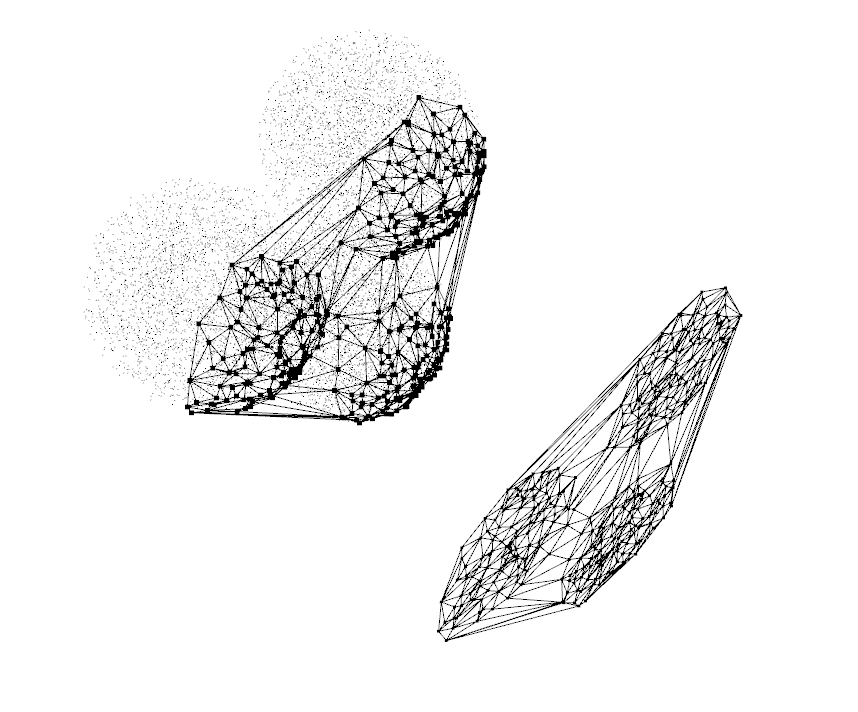
\includegraphics[width=0.6\textwidth]{../../images/3d_pareto_front_delaunay_triangulation.png}
    \caption[]{%
      This images shows a three-dimensional domain constructed by three uniform ball distributions and its triangulated Pareto frontier.
      First, the Pareto frontier has been projected onto the two-dimensional hyperplane with normal $n=\begin{pmatrix}1 & 1 & 1\end{pmatrix}$.
      Then the Delaunay algorithm was used to generate the triangulation.
    }
    \label{fig:pareto-delaunay-test}
  \end{figure*}
  \begin{figure*}
    \center
    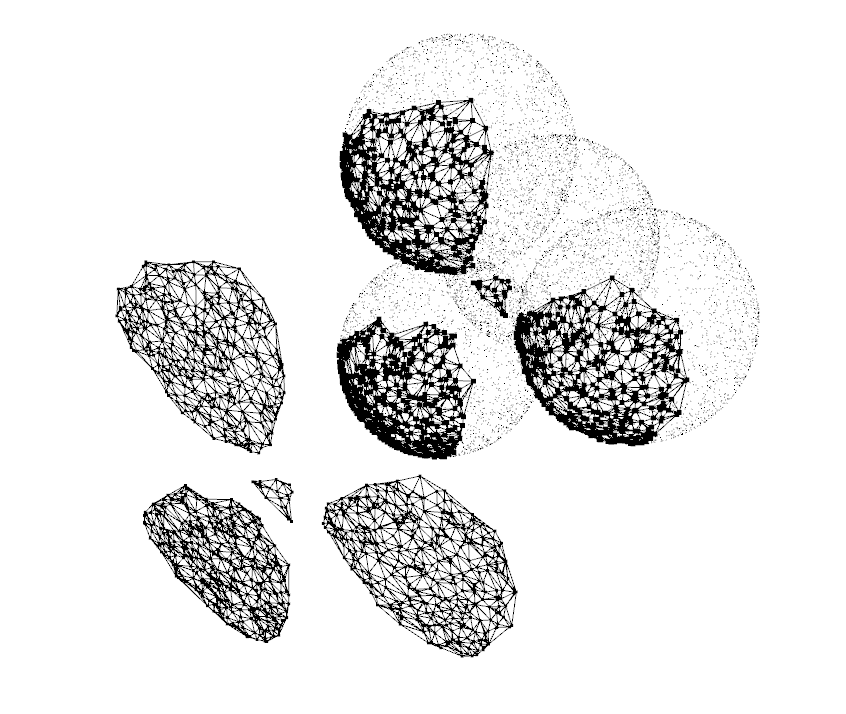
\includegraphics[width=0.6\textwidth]{../../images/3d_pareto_front_tessellation_01.png}
    \caption[]{%
      This images shows a three-dimensional domain constructed by four overlapping uniform sphere distributions and its triangulated Pareto frontier.
      First, the Pareto frontier has been projected onto the two-dimensional hyperplane with normal $n=\begin{pmatrix}1 & 1 & 1\end{pmatrix}$.
      Then the Delaunay algorithm was used to generate the triangulation.
      At the end, the statistical heuristic removed connections with large distances to dispose of incontinuities.
    }
    \label{fig:test-scene-1}
  \end{figure*}
  \begin{figure*}
    \center
    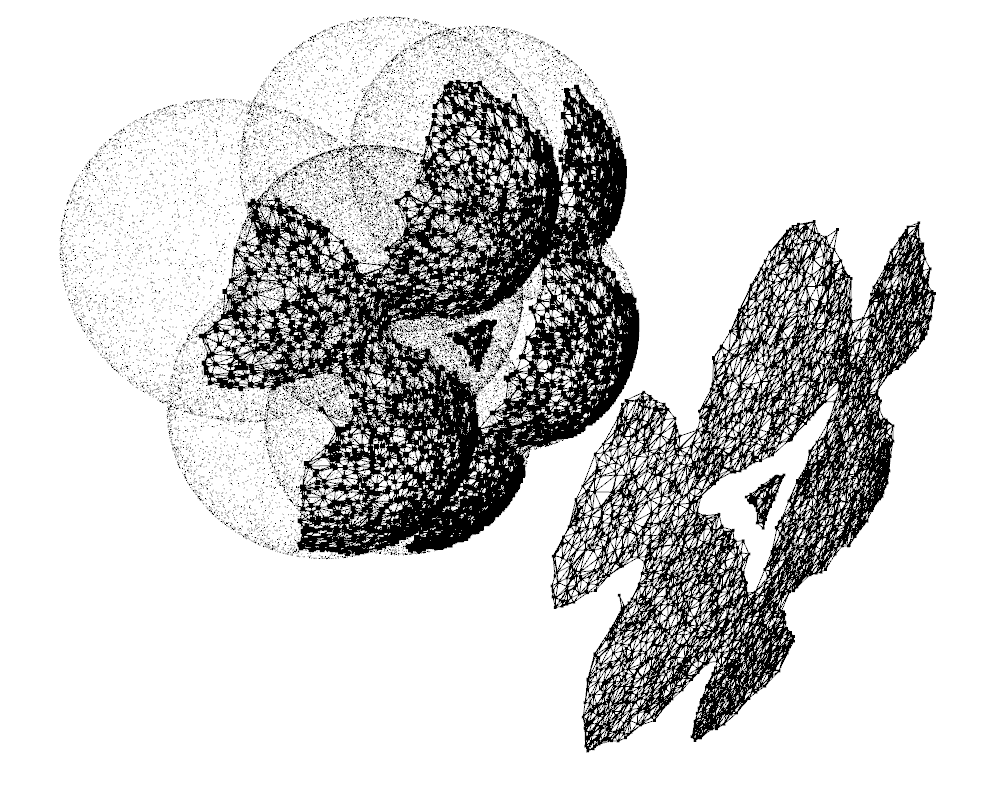
\includegraphics[width=0.6\textwidth]{../../images/3d_pareto_front_tessellation_02.png}
    \caption[]{%
      This images shows a three-dimensional domain constructed by seven overlapping uniform sphere distributions and its triangulated Pareto frontier.
      The same algorithm as in figure \ref{fig:test-scene-1} was used.
    }
    \label{fig:test-scene-2}
  \end{figure*}
% section results (end)
\end{document}